\chapter{Early Visual System}
\label{chap:visual_system}
This thesis focuses on modeling the \emph{primary visual cortex} (V1), a critical structure in early visual processing within the mammalian brain. V1 has been extensively studied for decades \citep{hubel1965receptive} and serves as a central focus in both experimental and computational neuroscience. In this chapter, we provide an overview of the most relevant components of the visual system for our modeling work. A comprehensive review of the entire visual system is beyond the scope of this thesis; for more detailed information, we refer the reader to standard neuroscience texts such as \citet{bear2020neuroscience} and \citet{goebel2004visual}, which also served as key references for this section.

\section{Neuron}
\label{sec:neuron}

The fundamental unit of neural processing in the brain is \emph{neuron}, a highly specialized cell adapted for the reception, integration, and transmission of electrochemical signals. Neurons differ from other cell types in both their unique morphology and functional properties, enabling rapid and complex information processing. Each neuron is composed of three principal components:

\begin{description}
    \item[Soma (Cell Body):] The \emph{soma} contains the nucleus and essential organelles responsible for protein synthesis, metabolic regulation, and overall cellular maintenance. It plays a crucial role in the integration of synaptic inputs received by the dendrites.

    \item[Dendrites:] \emph{Dendrites} extend from the soma and serve as the primary sites for receiving synaptic input from other neurons. Their extensive branching increases the surface area available for synaptic connections, allowing each neuron to integrate thousands of excitatory and inhibitory signals.

    \item[Axon:] The \emph{axon} is a specialized elongated projection responsible for transmitting electrical impulses to target neurons, often over long distances. It originates from \emph{axon hillock}, a region where the integrated membrane potential is evaluated and, if a threshold is reached, triggers an action potential and ends at \emph{axon terminals}, where communication with downstream neurons occurs through synapses.
\end{description}

The detailed anatomy of a neuron is illustrated in Figure \ref{fig:neuron}.

\begin{figure}
    \centering
    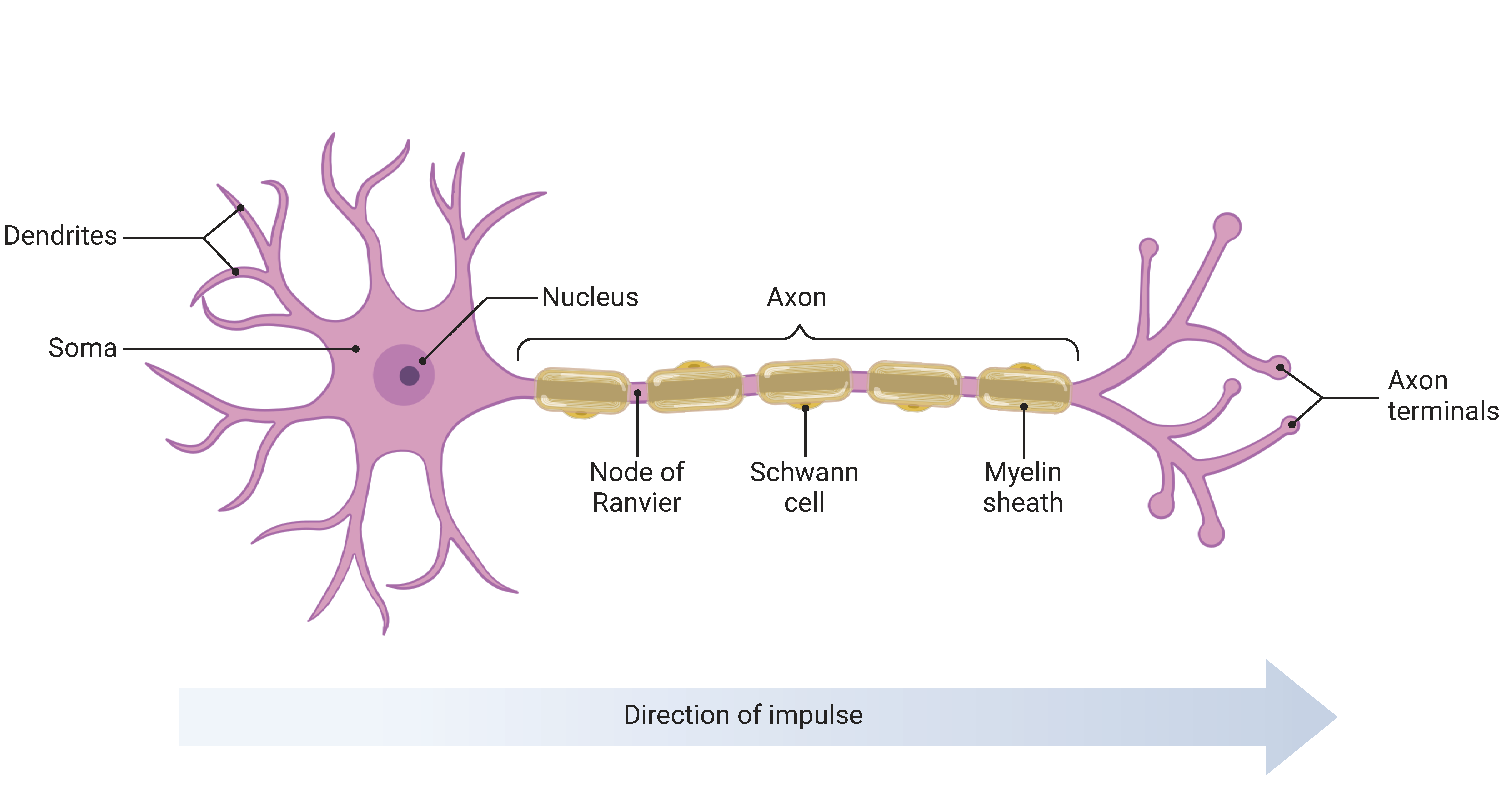
\includegraphics[width=\linewidth]{img/neuron_anatomy.pdf}
    \caption{\textbf{Neuron Anatomy.} A schematic illustration of the structural components of a typical neuron. "Created in BioRender. Beinhauer, D. (2025) https://BioRender.com/m351rlh".}
    \label{fig:neuron}
\end{figure}

Understanding the structure and function of individual neurons is essential, as these properties form the biological basis for the computational models used in this thesis. In the following sections, we build on this cellular foundation to explore how neurons are organized and interact within the primary visual cortex.

\subsection{Axon Overview}
\label{subsec:axon}

The axon is uniquely adapted for efficient signal propagation, enabled by specialized ion channels and structural proteins. At its terminal, the axon contains synaptic vesicles, membrane-bound structures that store \emph{neurotransmitters}, the chemical messengers essential for synaptic communication. Upon arrival of an action potential, these vesicles undergo exocytosis, releasing neurotransmitters into the synaptic cleft to influence the activity of the postsynaptic neuron. Common neurotransmitters include glutamate (the principal excitatory neurotransmitter in the central nervous system), gamma-aminobutyric acid (GABA; the primary inhibitory neurotransmitter), as well as glycine and acetylcholine, which play essential roles in both central and peripheral neural circuits.

Understanding the molecular mechanisms involved in neurotransmitter release and postsynaptic modulation is also vital from a computational modeling perspective. These processes govern signal integration and network dynamics, and their abstraction into model parameters such as synaptic weights and time constants plays a crucial role in biologically inspired simulations.

\subsection{Action Potential}
\label{subsec:action_potential}

The primary mechanism by which neurons transmit signals is the \emph{action potential}, a rapid, all-or-nothing electrical impulse that propagates along the axon. This process is governed by ion concentration gradients across the neuronal membrane and the resulting electrical potential differences.

At rest, neurons maintain a resting membrane potential of approximately $-65 \text{mV}$, established through selective ion permeability and the activity of the sodium-potassium ($\text{Na}^{+}/\text{K}^{+}$) pump. This pump actively transports $\text{Na}^{+}$ ions out of the cell and $\text{K}^{+}$ ions into the cell, preserving the concentration gradients required for neuronal excitability. Additional ions, including chloride ($\text{Cl}^{-}$) and calcium ($\text{Ca}^{2+}$), also contribute to membrane dynamics. In particular, most of these ions are more concentrated extracellularly, with the exception of $\text{K}^{+}$, which is more abundant within the neuron. Maintaining these ionic gradients accounts for a substantial portion of the brain's energy consumption.

The action potential unfolds in a stereotypical sequence of phases, as illustrated in Figure \ref{fig:action_potential}:

\begin{enumerate}
    \item \textbf{Generator Potential and Threshold Activation:} Synaptic inputs induce local changes in the membrane potential known as generator potentials. If the excitatory input is sufficient to depolarize the membrane to a threshold (typically around $-55 \text{mV}$), an action potential is initiated.
    
    \item \textbf{Rising Phase and Depolarization:} Voltage-gated $\text{Na}^{+}$ channels open, allowing a rapid influx of $\text{Na}^{+}$ ions. This drives the membrane potential sharply upward, occasionally overshooting to positive values.
    
    \item \textbf{Falling Phase and Repolarization:} As depolarization peaks, voltage-gated $\text{K}^{+}$ channels open and the $\text{Na}^{+}$ channels inactivate. The efflux of $\text{K}^{+}$ restores the membrane to a more negative potential.
    
    \item \textbf{Undershoot and Hyperpolarization:} $\text{K}^{+}$ conductance transiently exceeds baseline levels, causing the membrane potential to drop below the resting level, a phase called hyperpolarization.

    \item \textbf{Refractory Periods:}
    \begin{enumerate}
        \item \textbf{Absolute Refractory Period:} During this phase, $\text{Na}^{+}$ channels remain inactivated, rendering the neuron temporarily unresponsive to further stimulation.
        \item \textbf{Relative Refractory Period:} The membrane is still hyperpolarized, requiring a stronger stimulus than usual to trigger another action potential.
    \end{enumerate}
\end{enumerate}

\begin{figure}
    \centering
    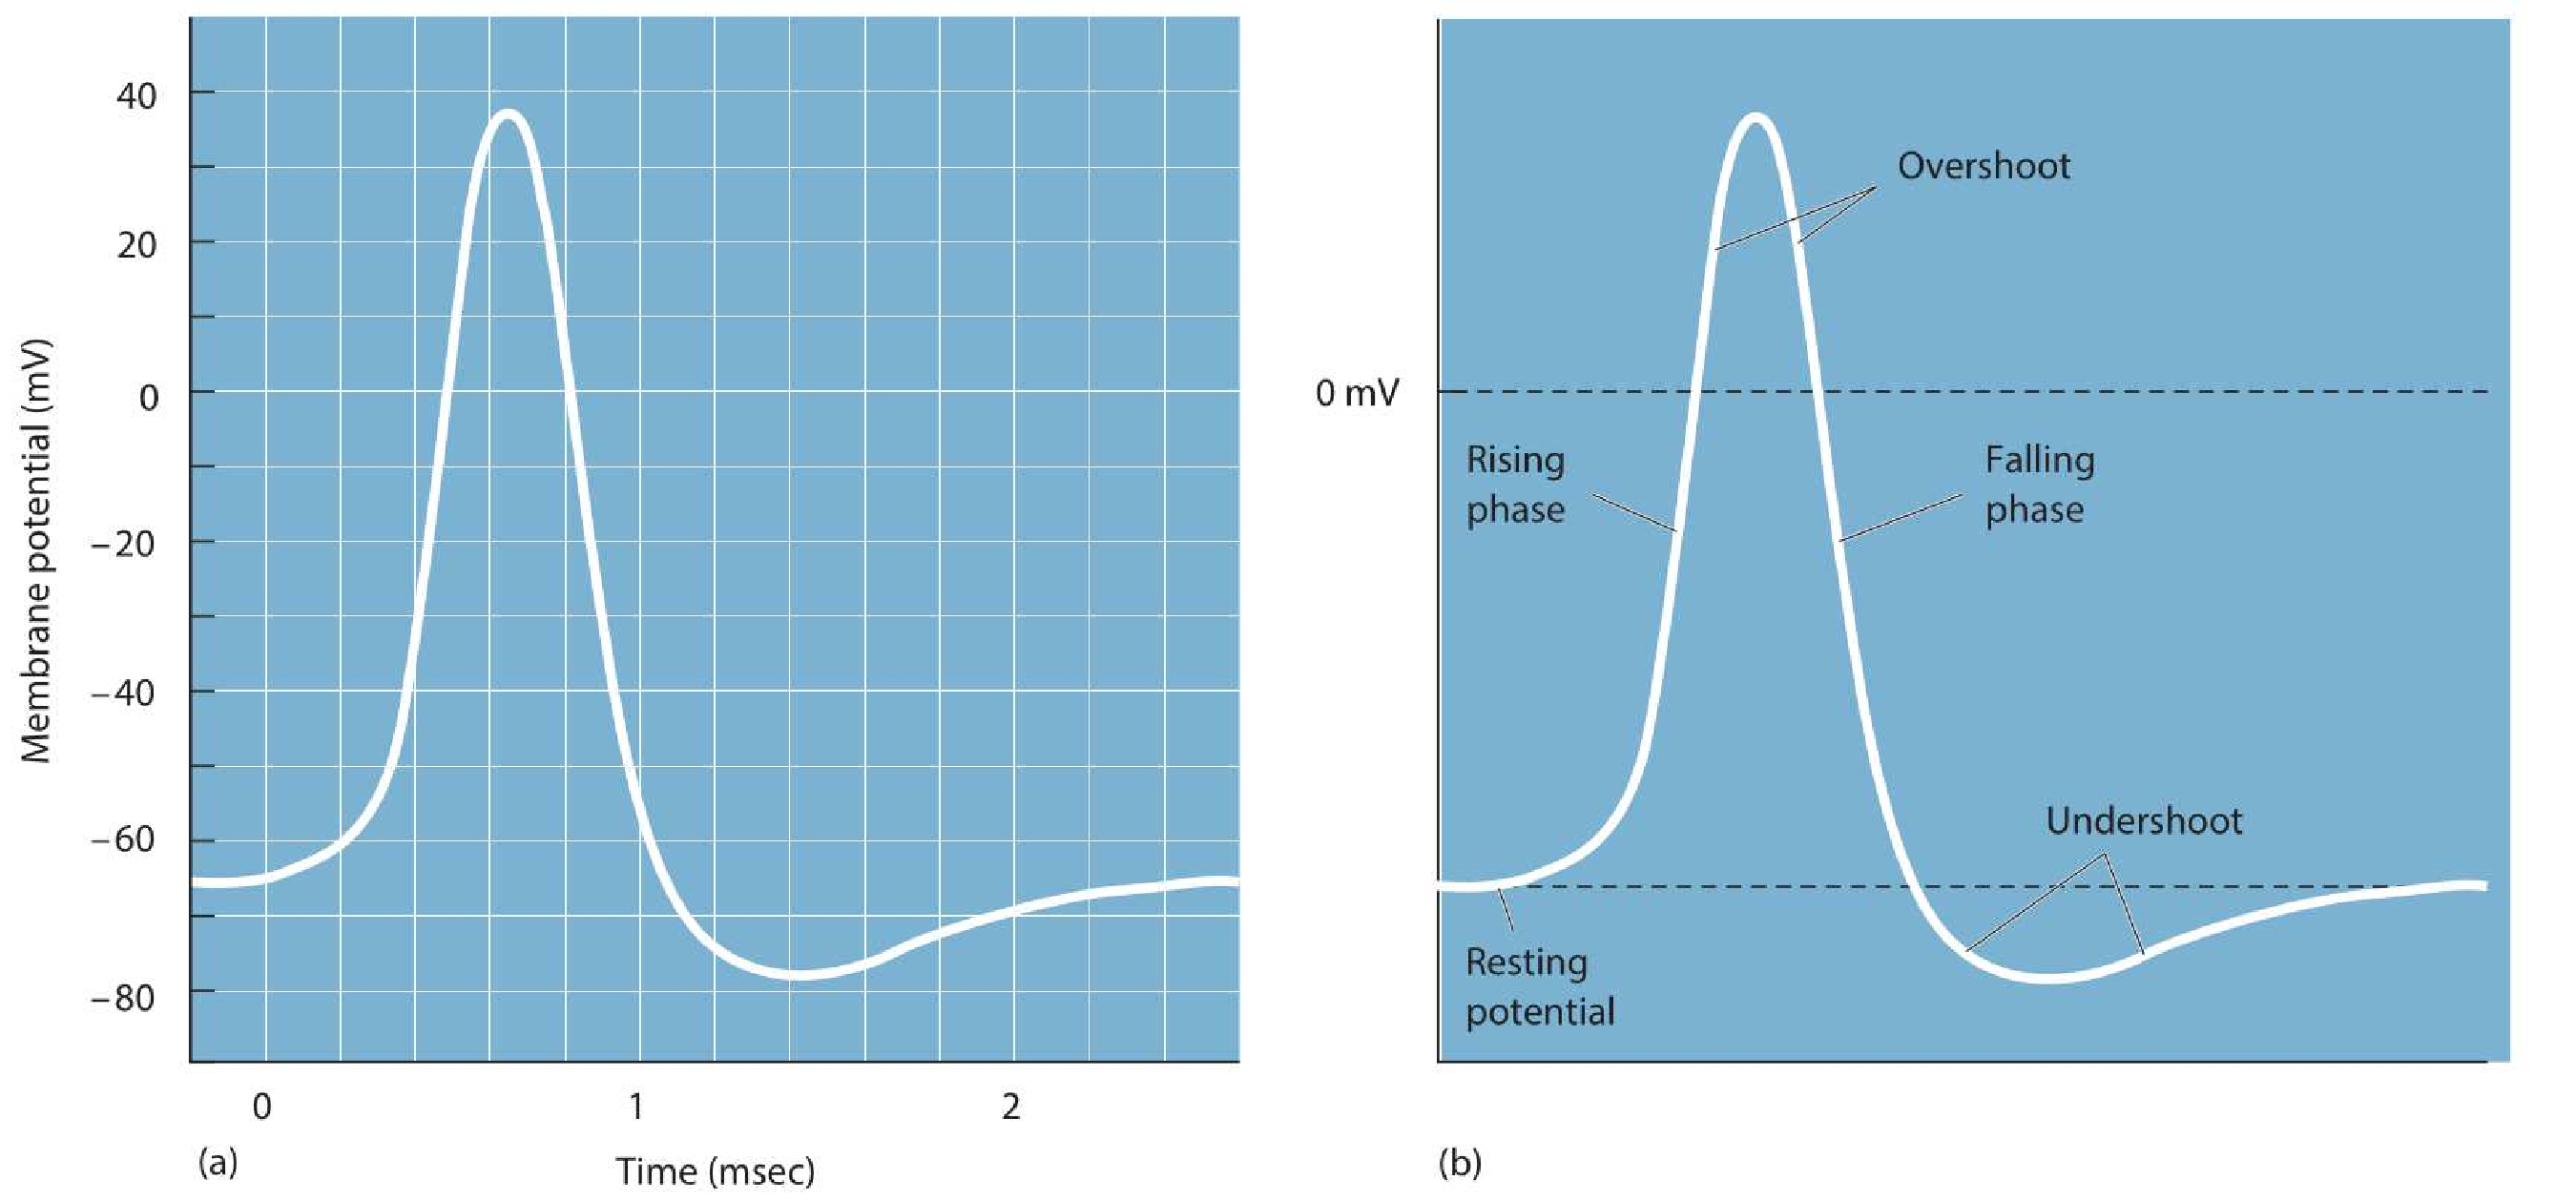
\includegraphics[width=\linewidth]{img/action_potential.pdf}
    \caption{\textbf{An action potential.} \textbf{a)} Oscilloscope trace of an action potential. \textbf{b)} Annotated phases of an action potential. The figure and the labels are taken from \emph{Neuroscience} (\citet{bear2020neuroscience}, 3rd Edition, p. 77).}
    \label{fig:action_potential}
\end{figure}

From a modeling point of view, the stereotyped threshold-based firing of neurons offers a basis for simplifying complex electrophysiological dynamics into discrete spiking models such as the leaky integration-and-fire model. These abstractions are commonly used in computational neuroscience to simulate neuronal behavior across large-scale networks.

\subsection{Axonal Conduction and Myelination}
\label{subsec:axonal_conduction}

Efficient transmission of action potentials across long axons is essential for rapid neural communication. The speed of conduction is significantly enhanced by \emph{myelination}, in which oligodendrocytes (in the central nervous system) and Schwann cells (in the peripheral nervous system) wrap the axons in layers of lipid-rich myelin. This insulation reduces ion leakage and allows \emph{saltatory conduction}, in which the action potential "jumps" between exposed regions of the axon known as \emph{nodes of Ranvier}. These nodes concentrate voltage-gated ion channels, supporting the regeneration of the action potential at regular intervals. This mechanism substantially increases the speed of transmission of the signal, particularly in long-range axonal projections. This structure is depicted in Figure \ref{fig:neuron}.

\subsection{Synaptic Transmission}
\label{subsec:synaptic_transmission}

At the axon terminal, the arrival of an action potential triggers the release of neurotransmitters stored in synaptic vesicles. This process, known as \emph{synaptic transmission}, unfolds through the following sequence:

\begin{enumerate}
    \item \textbf{Calcium Influx:} Voltage-gated $\text{Ca}^{2+}$ channels open, allowing $\text{Ca}^{2+}$ ions to enter the presynaptic terminal.
    \item \textbf{Vesicle Fusion and Neurotransmitter Release:} The increase in intracellular $\text{Ca}^{2+}$ concentration triggers vesicle fusion with the presynaptic membrane and subsequent neurotransmitter exocytosis.
    \item \textbf{Receptor Activation:} Neurotransmitters diffuse across the synaptic cleft and bind to specific receptors on the postsynaptic membrane, modulating the excitability of the postsynaptic neuron.
\end{enumerate}

Synapses can be broadly classified on the basis of their functional effects:

\begin{description}
    \item[Excitatory synapses:] Promote depolarization of the postsynaptic membrane, increasing the likelihood of generation of action potential.
    \item[Inhibitory synapses:] Induce hyperpolarization, decreasing the likelihood of postsynaptic firing.
\end{description}

This delicate balance between excitation and inhibition is fundamental for the function of neural circuits and underlies complex processes such as sensory perception, motor coordination, and cognition. In computational modeling, excitatory and inhibitory connections form the core of simulated network dynamics and are typically implemented using weighted synaptic interactions that modulate the state of artificial neurons in time.

\section{General Structure of the Early Visual System}
\label{sec:general_structure}

Almost half of the human brain is dedicated to visual processing, highlighting the importance of vision in human cognition and behavior. The initial stages of this processing occur within \emph{early visual system}.

Light from the environment enters the eye and passes through its complex optical components, ultimately reaching the retina a thin layer of neural tissue at the back of the eye. The retina not only detects light, but also performs the first stages of visual information processing. Signals from the retina travel along the optic nerve to the optic chiasm, where input from the visual fields is reorganized. The signal then continues through the optic tract to the \emph{lateral geniculate nucleus} (LGN) of the thalamus, a crucial relay station that refines and filters the input before sending it to the cortex.

From the LGN, visual information is transmitted through optical radiations to the \emph{primary visual cortex} (V1), the first cortical area exclusively dedicated to visual processing. V1 performs fundamental computations such as edge detection, orientation selectivity, and spatial frequency tuning (\citet{bear2020neuroscience}). From there, signals are sent to higher-order visual areas that support more complex functions, including object recognition, motion analysis, and depth perception.

From a computational point of view, the early visual system provides a powerful model of hierarchical processing. Each stage from the retina to V1 performs increasingly complex transformations of sensory input, extracting spatial, temporal, and contextual features. Many principles underlying modern artificial and biologically inspired neural networks, such as receptive fields, feedforward and feedback loops, and parallel processing, can be traced back to the structure and function of these early visual pathways. In the following sections, we examine these components in more detail, with a particular focus on the transformations that occur in the retina, LGN, and V1, laying the groundwork for computational models that emulate these processes.

\section{Eye}
\label{sec:eye}

The eye acts as a sophisticated optical system that captures electromagnetic radiation (light), modulates it through a series of specialized structures, and focuses it onto the retina. Key components including the cornea, lens, iris, and pupil work together to regulate light entry and ensure proper focusing. A detailed anatomical overview is presented in Figure~\ref{fig:eye} and elaborated upon in \citet{snell2013clinical}.

\begin{figure}
    \centering
    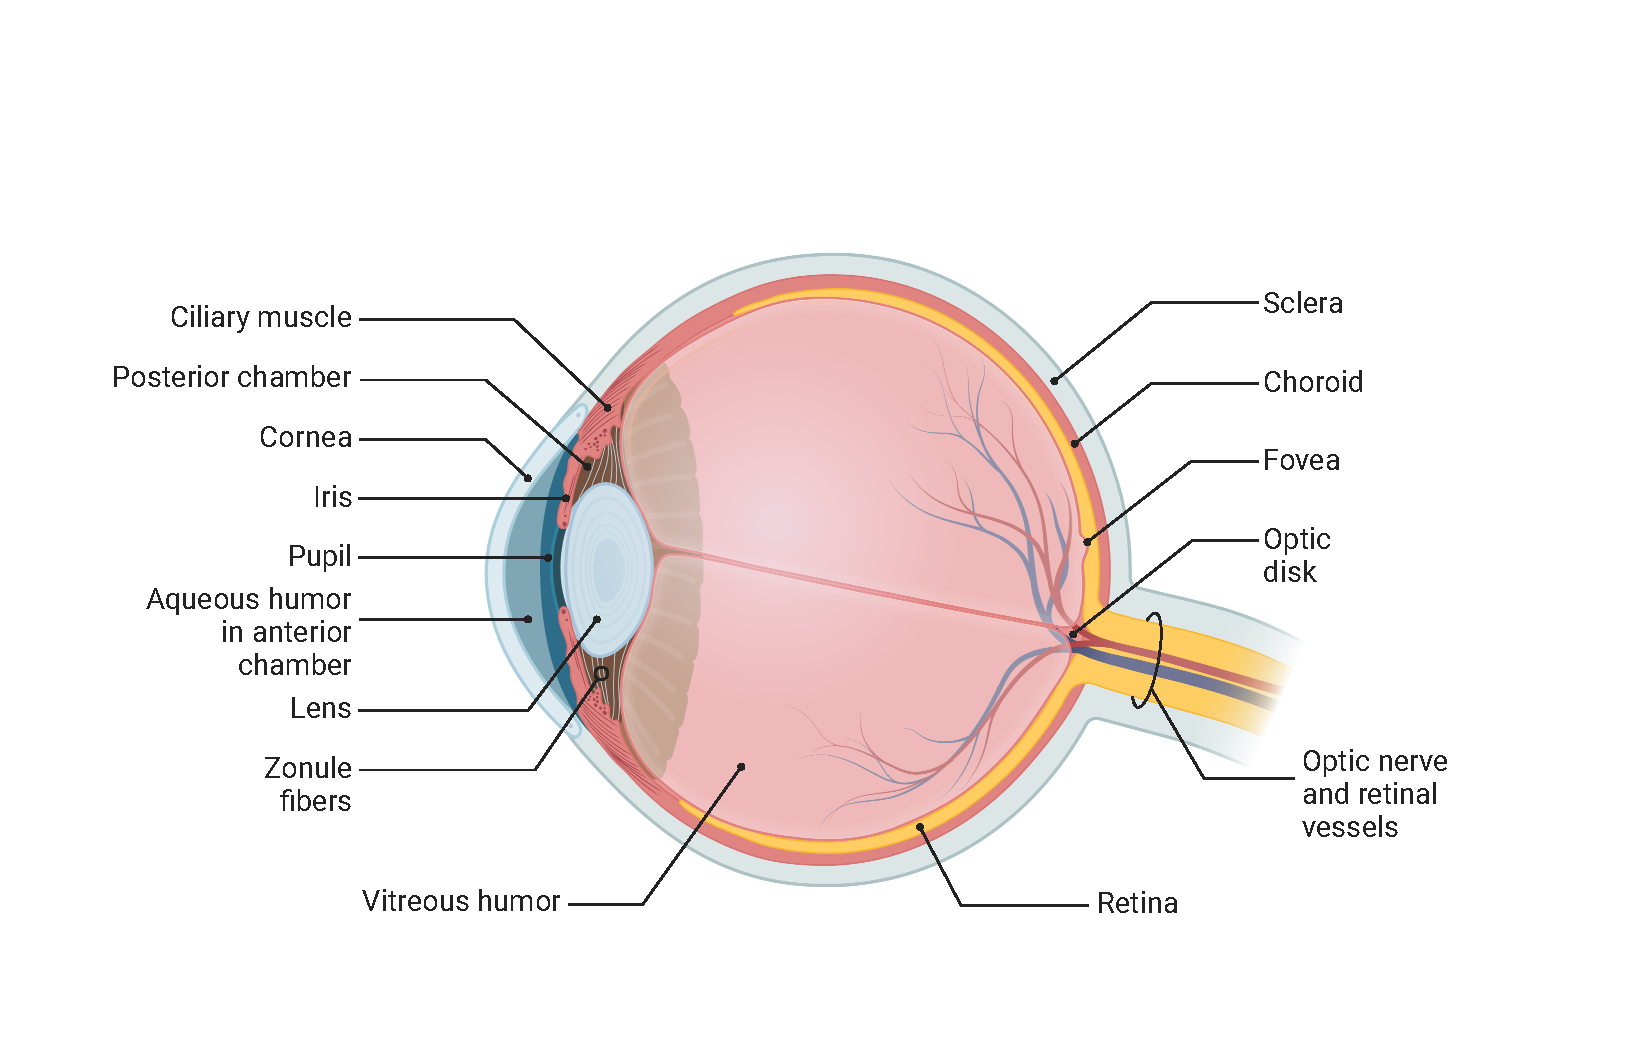
\includegraphics[width=\linewidth]{img/eye.pdf}
    \caption{\textbf{An anatomy of an eye.} Illustration based on (\citet{bear2020neuroscience}, 3rd Edition, p. 283). "Created in BioRender. Beinhauer, D. (2025) https://BioRender.com/8n8epge".}
    \label{fig:eye}
\end{figure}


\subsection{Retina}
\label{subsec:retina}

Beyond capturing light, a key function of the eye is to convert optical stimuli into neural signals for transmission to the brain. This conversion is carried out by the retina a multilayered neural tissue composed of several specialized cell types organized into distinct layers. These include \emph{photoreceptors}, \emph{bipolar cells}, \emph{horizontal cells}, \emph{amacrine cells}, and \emph{ganglion cells}, as shown in Figure \ref{fig:retina_anatomy}.

\begin{figure}
    \centering
    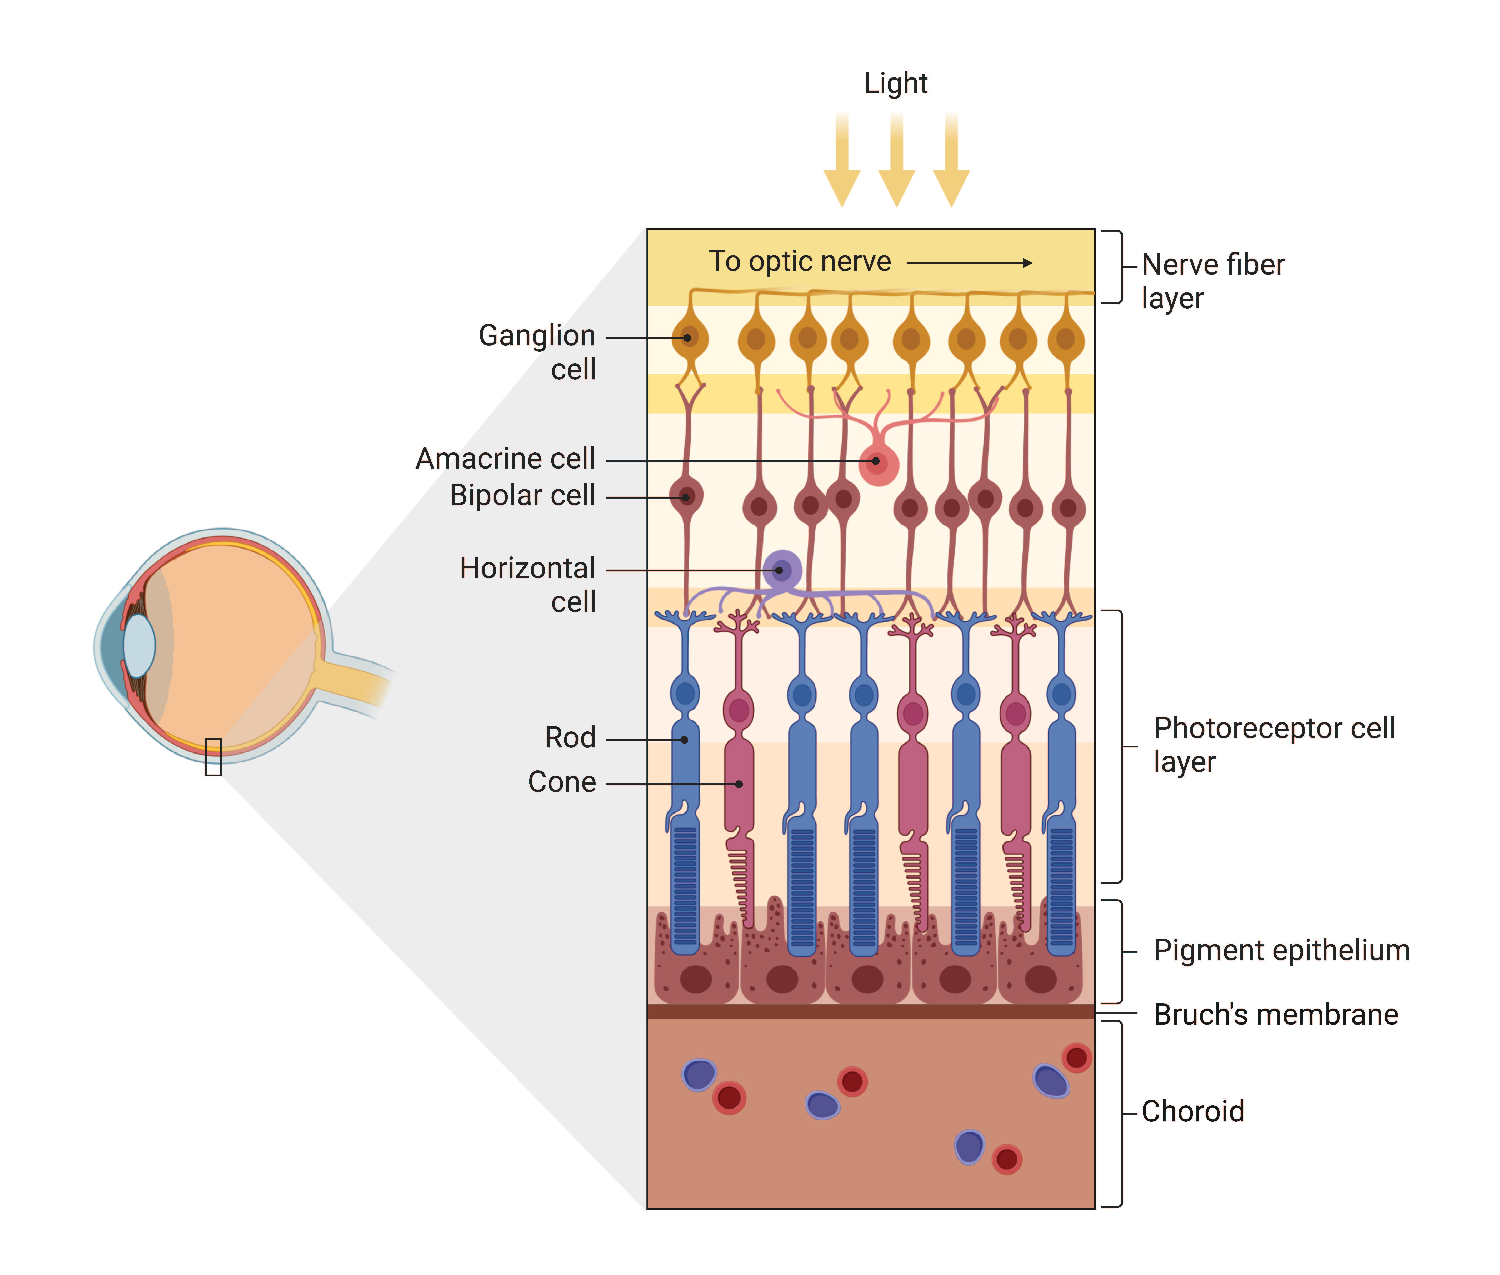
\includegraphics[width=\linewidth]{img/retina_anatomy.pdf}
    \caption{\textbf{Layered anatomy of the retina.} Adapted from (\citet{schwartz1991principles}, 4th Edition, p. 436) and (\citet{purves2019neurosciences}, 6th Edition, p. 239). "Created in BioRender. Beinhauer, D. (2025) https://BioRender.com/oy5qz9v".}
    \label{fig:retina_anatomy}
\end{figure}

Visual processing begins with \emph{photoreceptors}, which include \emph{rods} and \emph{cones}. These cells transduce light into electrical signals via photochemical reactions in their outer segments. Rods are highly sensitive and support scotopic (low-light) vision, whereas cones enable color perception and high-acuity vision under photopic (well-lit) conditions. Their spatial distribution is nonuniform: the central region of the retina - \emph{fovea} contains a dense concentration of cones, while rods dominate the peripheral retina. A \emph{blind spot} exists in the optic disc, where ganglion cell axons exit the eye to form the optic nerve; this region does not contain photoreceptors.    

Upon light activation, photoreceptors undergo hyperpolarization, which reduces their release of the neurotransmitter \emph{glutamate}. This change is detected by \emph{bipolar cells}, which relays the signal deeper into the retina. Most retinal neurons, except for ganglion cells, communicate using graded potentials rather than action potentials, allowing fine-grained signal modulation.

Approximately 10 million bipolar cells integrate input from around 125 million photoreceptors. Their connectivity patterns vary by cell type and location in the retina. \emph{Horizontal cells} provide lateral inhibition by integrating the input of multiple photoreceptors, thus enhancing the contrast at the earliest stage of processing.

Bipolar cells are functionally categorized into the \emph{ON} and \emph{OFF} types, depending on their response to light. ON bipolar cells depolarize in response to light onset, while OFF bipolar cells hyperpolarize. Both types exhibit \emph{center-surround receptive fields}, which support spatial contrast detection. Horizontal cells contribute to this mechanism by mediating inhibitory signals from surrounding photoreceptors. Figure \ref{fig:on_off_cells} illustrates these pathways for ON bipolar cells.

\begin{figure}
    \centering
    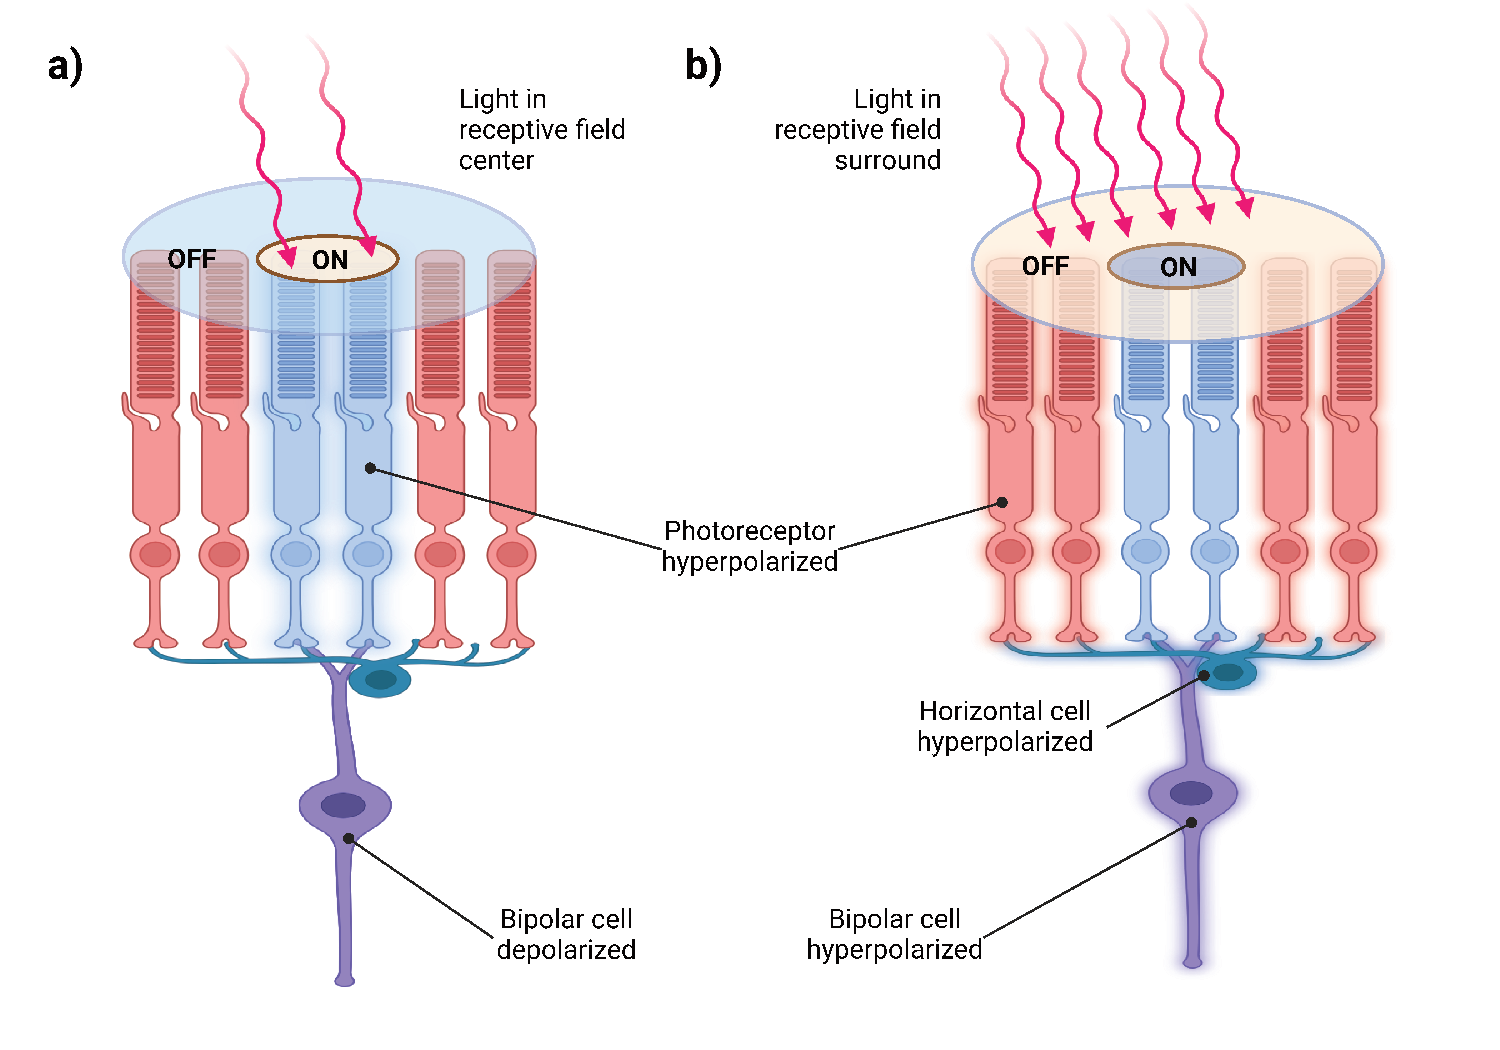
\includegraphics[width=\linewidth]{img/on_off_cells.pdf}
    \caption{\textbf{Direct and indirect pathways from photoreceptors to bipolar cells.} \textbf{a)} An ON bipolar cell depolarizes in response to light in the center of its receptive field. \textbf{b)} The same cell hyperpolarizes in response to surround stimulation. Based on \emph{Neuroscience} (\citet{bear2020neuroscience}, 3rd Edition, p. 300). "Created in BioRender. Beinhauer, D. (2025) https://BioRender.com/bpeqbrd".}
    \label{fig:on_off_cells}
\end{figure}

The final stage of retinal processing occurs in the \emph{ganglion cells}, the only retinal neurons that generate action potentials. These cells receive input from bipolar and \emph{amacrine cells}, preserving the center-surround receptive field structure. Their axons converge to form the \emph{optic nerve}, which transmits encoded visual information to the LGN.

This layered processing within the retina fundamentally shapes the signals that reach the cortical areas. Mechanisms such as lateral inhibition, center-surround receptive fields, and ON/OFF channel segregation serve as early examples of efficient, parallelized feature extraction, an inspiration for many biologically plausible models in computational neuroscience. These transformations determine the structure of the input received by the higher visual areas and influence how visual scenes are encoded and interpreted. Understanding these mechanisms is therefore essential when designing models that aim to replicate the spatial and temporal dynamics of visual processing observed in the brain.

\section{Lateral Geniculate Nucleus}
\label{sec:lgn}
The next major processing stage in the visual pathway is \emph{Lateral Geniculate Nucleus (LGN)}, a subcortical relay structure located within the thalamus. The LGN acts as the main gateway to the cortex, receiving input from retinal ganglion cells and transmitting these signals to the primary visual cortex (V1) via the optic radiations. Given V1's critical role in conscious visual perception, lesions anywhere along this pathway, from the retina to the LGN to V1, can result in localized or complete visual deficits, illustrating the hierarchical and modular organization of the visual system.

In particular, the LGN receives more input from the cortex than from the retina itself. This corticothalamic feedback, predominantly originating in V1, is believed to modulate LGN activity through top-down influences such as attention, expectation, and dynamic gain control. These mechanisms reflect the brain's predictive and adaptive coding strategies, supporting context-dependent processing rather than passive transmission.

Structurally, the LGN is composed of six distinct layers, each of which processes input from only one eye, maintaining strict monocular segregation. These layers are organized to preserve the retinotopy, ensuring spatial continuity of the visual field. Functionally, the LGN supports multiple parallel processing streams: magnocellular layers (M) encode motion and low-spatial-frequency information; parvocellular layers (P) process color and fine spatial details; and koniocellular layers contribute additional chromatic and feature-specific inputs. LGN neurons retain the receptive field structure of the center surrounding the retinal ganglion cells, enhancing contrast and edge representation.

This layered and functionally diverse architecture makes the LGN more than a simple relay station. It serves as a dynamic filter that integrates sensory input with cortical modulation.

\section{Primary Visual Cortex}
\label{sec:v1}

The primary visual cortex (V1), located in the occipital lobe, represents the first cortical stage dedicated to visual information processing. It extracts fundamental features from visual stimuli, including orientation, spatial frequency, motion, and color. Following this initial analysis, visual information is funneled into two major processing streams: the parvocellular (P) pathway, which emphasizes high resolution spatial detail and object recognition, and the magnocellular (M) pathway, specialized for motion detection and temporal dynamics.(as mentioned in Section \ref{sec:lgn}).

V1 is organized into six histologically distinct layers, conventionally labeled with
Roman numerals. The primary input from the LGN is directed to layer IV, which is divided into four sublayers (IVA, IVB, IVC$\alpha$, and IVC$\beta$). Layer IVC, 
in particular, serves as the principal recipient of LGN projections, processing
monocular input before distributing signals to layers II and III, where binocular
integration occurs. From these layers, information is transmitted to higher-order 
visual areas such as V2, V3, and beyond, enabling progressively more complex visual
computations. Layers V and VI are primarily involved in feedback connections, 
modulating activity within earlier visual processing stages.

Intricate interlaminar connectivity is a hallmark of V1, particularly within layer IV, 
where excitatory and inhibitory neurons form recurrent circuits that refine feature
detection. Although inhibitory interneurons predominantly exert influence within their
respective layers, excitatory pyramidal neurons extend projections across multiple
layers, facilitating hierarchical processing.

A critical organizational feature of V1 is \emph{retinotopy}, where the spatial
arrangement of neurons preserves the topographical representation of the retina. 
However, this mapping is nonuniform, with a disproportionately large cortical
representation of the fovea relative to peripheral visual fields, reflecting the
greater density of photoreceptors in central vision.

\subsection{Receptive field properties of V1 cells}
\label{subsec:receptive_field}
V1 neurons exhibit selectivity for different stimulus attributes, forming
overlapping computational maps that encode various aspects of the visual scene. 
These selectivities include:

\begin{description}
    \item[Orientation selectivity:] Neurons in the layer IVC ($\alpha$ and $\beta$) begin to exhibit elongated receptive fields, departing from the concentric organization observed in earlier visual processing stages. This transformation enables sensitivity to the orientation of edges and lines, with each neuron preferentially responding to a specific angular configuration. The arrangement of orientation-selective neurons follows a columnar organization in which cells with similar orientation preferences are clustered.
    \begin{description}
        \item[Simple Cells:] Simple cells demonstrate selectivity not only for orientation 
        but also for the precise spatial positioning of an edge within their receptive field. 
        Their response properties are derived from the summation of inputs from multiple LGN cells arranged antagonistically.
        \item[Complex Cells:] Complex cells, in contrast, maintain orientation selectivity but are less constrained by stimulus position within their receptive field. They 
        integrate signals from multiple simple cells, resulting in robust responses to oriented edges regardless of their exact location.
    \end{description}
    \item[Direction Selectivity:] Certain V1 neurons are tuned to the direction of motion, 
    responding preferentially to stimuli moving in a specific trajectory. These neurons play a crucial role in encoding motion dynamics and contribute to higher-order motion perception.
    \item[Binocularity:] While neurons in layer IV process monocular input primarily, subsequent layers integrate signals from both eyes, enabling binocular depth perception through mechanisms such as disparity tuning.
    \item[Additional Functional Specializations:] Beyond orientation and motion selectivity, 
    subsets of V1 neurons are specialized for processing stereoscopic depth, color opponency, 
    and feedback modulation from higher-order cortical areas.
\end{description}

\section{Extrastriate Visual Cortex}
\label{sec:extrastriate}

Beyond V1, visual processing continues in a network of extrastriate cortical regions
that extract increasingly abstract features of the visual scene. These areas include
V2, V3, V4, and MT (middle temporal area), each contributing to distinct aspects of
perception such as object recognition, motion tracking, and depth analysis. Damage
to these regions does not typically result in complete blindness, but instead leads to
specific deficits, such as achromatopsia (loss of color perception) or motion blindness
(inability to perceive fluid motion), depending on the affected region.
